% ============================================
% PARTE 3: EJERCICIOS PROPUESTOS
% ============================================

\section{Ejercicios Propuestos}

Ahora es tu turno de practicar. Resuelve los siguientes ejercicios aplicando los conceptos aprendidos. Todas las soluciones están incluidas al final para que puedas verificar tu trabajo.

% ============================================
% EJERCICIO 1: Distancia entre dos puntos
% ============================================

\begin{ejercicio}[Distancia entre dos puntos - Nivel BÁSICO]
Calcula la distancia entre los siguientes pares de puntos:

\textbf{a)} $P(1, 2)$ y $Q(4, 6)$

\textbf{b)} $A(-3, 5)$ y $B(2, -7)$

\textbf{c)} $M(0, 0)$ y $N(-6, 8)$
\end{ejercicio}

\begin{solucion}
\textbf{Inciso a):}

Aplicamos la fórmula de distancia:
\[
d = \sqrt{(x_2 - x_1)^2 + (y_2 - y_1)^2} = \sqrt{(4-1)^2 + (6-2)^2} = \sqrt{9 + 16} = \sqrt{25} = 5
\]

\textbf{Respuesta:} $\boxed{d = 5 \text{ unidades}}$

\textbf{Inciso b):}

\[
d = \sqrt{(2-(-3))^2 + (-7-5)^2} = \sqrt{5^2 + (-12)^2} = \sqrt{25 + 144} = \sqrt{169} = 13
\]

\textbf{Respuesta:} $\boxed{d = 13 \text{ unidades}}$

\textbf{Inciso c):}

\[
d = \sqrt{(-6-0)^2 + (8-0)^2} = \sqrt{36 + 64} = \sqrt{100} = 10
\]

\textbf{Respuesta:} $\boxed{d = 10 \text{ unidades}}$

\begin{nota}
El inciso c) es especialmente simple porque uno de los puntos es el origen. El inciso a) y c) resultan en triángulos pitagóricos conocidos: 3-4-5 y 6-8-10.
\end{nota}
\end{solucion}

% ============================================
% EJERCICIO 2: Punto medio
% ============================================

\begin{ejercicio}[Punto medio de un segmento - Nivel BÁSICO]
Encuentra el punto medio del segmento que une los siguientes pares de puntos:

\textbf{a)} $A(2, 8)$ y $B(10, 4)$

\textbf{b)} $P(-5, 3)$ y $Q(7, -1)$

\textbf{c)} $M(0, 6)$ y $N(8, 0)$
\end{ejercicio}

\begin{solucion}
\textbf{Inciso a):}

Aplicamos la fórmula del punto medio:
\[
M = \left( \frac{x_1 + x_2}{2}, \frac{y_1 + y_2}{2} \right) = \left( \frac{2 + 10}{2}, \frac{8 + 4}{2} \right) = \left( \frac{12}{2}, \frac{12}{2} \right) = (6, 6)
\]

\textbf{Respuesta:} $\boxed{M = (6, 6)}$

\textbf{Inciso b):}

\[
M = \left( \frac{-5 + 7}{2}, \frac{3 + (-1)}{2} \right) = \left( \frac{2}{2}, \frac{2}{2} \right) = (1, 1)
\]

\textbf{Respuesta:} $\boxed{M = (1, 1)}$

\textbf{Inciso c):}

\[
M = \left( \frac{0 + 8}{2}, \frac{6 + 0}{2} \right) = (4, 3)
\]

\textbf{Respuesta:} $\boxed{M = (4, 3)}$

\begin{center}
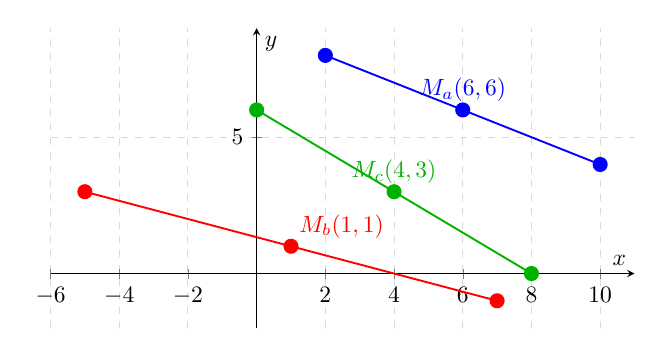
\begin{tikzpicture}[scale=0.85]
\begin{axis}[
    width=0.85\textwidth,
    height=0.5\textwidth,
    axis lines=middle,
    xlabel={$x$},
    ylabel={$y$},
    xmin=-6, xmax=11,
    ymin=-2, ymax=9,
    grid=major,
    grid style={dashed, gray!30},
]

% Inciso a)
\addplot[thick, color=blue] coordinates {(2,8) (10,4)};
\addplot[only marks, mark=*, mark size=3pt, color=blue] coordinates {(2,8) (10,4) (6,6)};
\node[above, blue] at (axis cs:6,6) {$M_a(6,6)$};

% Inciso b)
\addplot[thick, color=red] coordinates {(-5,3) (7,-1)};
\addplot[only marks, mark=*, mark size=3pt, color=red] coordinates {(-5,3) (7,-1) (1,1)};
\node[above right, red] at (axis cs:1,1) {$M_b(1,1)$};

% Inciso c)
\addplot[thick, color=green!70!black] coordinates {(0,6) (8,0)};
\addplot[only marks, mark=*, mark size=3pt, color=green!70!black] coordinates {(0,6) (8,0) (4,3)};
\node[above, green!70!black] at (axis cs:4,3) {$M_c(4,3)$};

\end{axis}
\end{tikzpicture}
\end{center}
\end{solucion}

% ============================================
% EJERCICIO 3: Pendiente
% ============================================

\begin{ejercicio}[Pendiente de una recta - Nivel BÁSICO-INTERMEDIO]
Calcula la pendiente de la recta que pasa por los siguientes pares de puntos:

\textbf{a)} $A(1, 3)$ y $B(5, 11)$

\textbf{b)} $P(-2, 4)$ y $Q(3, -6)$

\textbf{c)} $M(7, 2)$ y $N(7, 9)$
\end{ejercicio}

\begin{solucion}
\textbf{Inciso a):}

\[
m = \frac{y_2 - y_1}{x_2 - x_1} = \frac{11 - 3}{5 - 1} = \frac{8}{4} = 2
\]

\textbf{Respuesta:} $\boxed{m = 2}$ (la recta sube 2 unidades por cada unidad horizontal)

\textbf{Inciso b):}

\[
m = \frac{-6 - 4}{3 - (-2)} = \frac{-10}{5} = -2
\]

\textbf{Respuesta:} $\boxed{m = -2}$ (la recta baja 2 unidades por cada unidad horizontal)

\textbf{Inciso c):}

\[
m = \frac{9 - 2}{7 - 7} = \frac{7}{0}
\]

Como la división por cero no está definida, la pendiente es \textbf{indefinida}.

\textbf{Respuesta:} $\boxed{\text{Pendiente indefinida (recta vertical)}}$

\begin{nota}
Cuando dos puntos tienen la misma coordenada $x$ (como en el inciso c), la recta es vertical y su pendiente es indefinida. Su ecuación es de la forma $x = k$ (en este caso, $x = 7$).
\end{nota}

\begin{center}
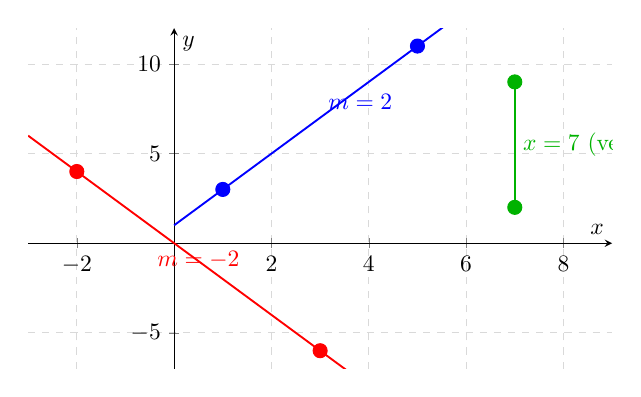
\begin{tikzpicture}[scale=0.85]
\begin{axis}[
    width=0.85\textwidth,
    height=0.55\textwidth,
    axis lines=middle,
    xlabel={$x$},
    ylabel={$y$},
    xmin=-3, xmax=9,
    ymin=-7, ymax=12,
    grid=major,
    grid style={dashed, gray!30},
]

% Inciso a) m=2
\addplot[thick, color=blue, domain=0:6] {2*x + 1};
\addplot[only marks, mark=*, mark size=3pt, color=blue] coordinates {(1,3) (5,11)};
\node[above right, blue] at (axis cs:3,7) {$m=2$};

% Inciso b) m=-2
\addplot[thick, color=red, domain=-3:4] {-2*x};
\addplot[only marks, mark=*, mark size=3pt, color=red] coordinates {(-2,4) (3,-6)};
\node[below, red] at (axis cs:0.5,0) {$m=-2$};

% Inciso c) vertical
\addplot[thick, color=green!70!black] coordinates {(7,2) (7,9)};
\addplot[only marks, mark=*, mark size=3pt, color=green!70!black] coordinates {(7,2) (7,9)};
\node[right, green!70!black] at (axis cs:7,5.5) {$x=7$ (vertical)};

\end{axis}
\end{tikzpicture}
\end{center}
\end{solucion}

% ============================================
% EJERCICIO 4: Ecuación punto-pendiente
% ============================================

\begin{ejercicio}[Ecuación punto-pendiente - Nivel INTERMEDIO]
Encuentra la ecuación de la recta que satisface las siguientes condiciones y exprésala en forma pendiente-ordenada ($y = mx + b$):

\textbf{a)} Pasa por $P(3, 7)$ con pendiente $m = 4$

\textbf{b)} Pasa por $Q(-2, 5)$ con pendiente $m = -\frac{1}{2}$

\textbf{c)} Pasa por $R(0, -3)$ con pendiente $m = \frac{3}{4}$
\end{ejercicio}

\begin{solucion}
\textbf{Inciso a):}

Forma punto-pendiente:
\begin{align*}
y - y_1 &= m(x - x_1) \\
y - 7 &= 4(x - 3) \\
y - 7 &= 4x - 12 \\
y &= 4x - 5
\end{align*}

\textbf{Respuesta:} $\boxed{y = 4x - 5}$

\textbf{Inciso b):}

\begin{align*}
y - 5 &= -\frac{1}{2}(x - (-2)) \\
y - 5 &= -\frac{1}{2}(x + 2) \\
y - 5 &= -\frac{1}{2}x - 1 \\
y &= -\frac{1}{2}x + 4
\end{align*}

\textbf{Respuesta:} $\boxed{y = -\frac{1}{2}x + 4}$

\textbf{Inciso c):}

Como el punto es $(0, -3)$ (está en el eje $y$), este es directamente el punto de ordenada al origen ($b = -3$):
\begin{align*}
y - (-3) &= \frac{3}{4}(x - 0) \\
y + 3 &= \frac{3}{4}x \\
y &= \frac{3}{4}x - 3
\end{align*}

\textbf{Respuesta:} $\boxed{y = \frac{3}{4}x - 3}$

\begin{nota}
En el inciso c), como el punto dado tiene $x = 0$, podemos identificar directamente que $b = -3$, y la ecuación se simplifica a $y = mx + b = \frac{3}{4}x - 3$.
\end{nota}
\end{solucion}

% ============================================
% EJERCICIO 5: Ecuación dados dos puntos
% ============================================

\begin{ejercicio}[Ecuación dados dos puntos - Nivel INTERMEDIO]
Encuentra la ecuación de la recta que pasa por los siguientes pares de puntos. Expresa la respuesta en forma general ($Ax + By + C = 0$):

\textbf{a)} $A(2, 5)$ y $B(6, 13)$

\textbf{b)} $P(-1, 4)$ y $Q(3, -2)$

\textbf{c)} $M(4, 1)$ y $N(-2, 7)$
\end{ejercicio}

\begin{solucion}
\textbf{Inciso a):}

\textbf{Paso 1:} Calculamos la pendiente:
\[
m = \frac{13 - 5}{6 - 2} = \frac{8}{4} = 2
\]

\textbf{Paso 2:} Forma punto-pendiente con $A(2, 5)$:
\[
y - 5 = 2(x - 2) \quad \Rightarrow \quad y - 5 = 2x - 4 \quad \Rightarrow \quad y = 2x + 1
\]

\textbf{Paso 3:} Forma general:
\[
2x - y + 1 = 0
\]

\textbf{Respuesta:} $\boxed{2x - y + 1 = 0}$

\textbf{Inciso b):}

\textbf{Paso 1:} Pendiente:
\[
m = \frac{-2 - 4}{3 - (-1)} = \frac{-6}{4} = -\frac{3}{2}
\]

\textbf{Paso 2:} Forma punto-pendiente con $P(-1, 4)$:
\begin{align*}
y - 4 &= -\frac{3}{2}(x - (-1)) \\
y - 4 &= -\frac{3}{2}(x + 1) \\
y - 4 &= -\frac{3}{2}x - \frac{3}{2} \\
y &= -\frac{3}{2}x + \frac{5}{2}
\end{align*}

\textbf{Paso 3:} Forma general (multiplicamos por 2):
\begin{align*}
2y &= -3x + 5 \\
3x + 2y - 5 &= 0
\end{align*}

\textbf{Respuesta:} $\boxed{3x + 2y - 5 = 0}$

\textbf{Inciso c):}

\textbf{Paso 1:} Pendiente:
\[
m = \frac{7 - 1}{-2 - 4} = \frac{6}{-6} = -1
\]

\textbf{Paso 2:} Forma punto-pendiente con $M(4, 1)$:
\begin{align*}
y - 1 &= -1(x - 4) \\
y - 1 &= -x + 4 \\
y &= -x + 5
\end{align*}

\textbf{Paso 3:} Forma general:
\[
x + y - 5 = 0
\]

\textbf{Respuesta:} $\boxed{x + y - 5 = 0}$

\begin{center}
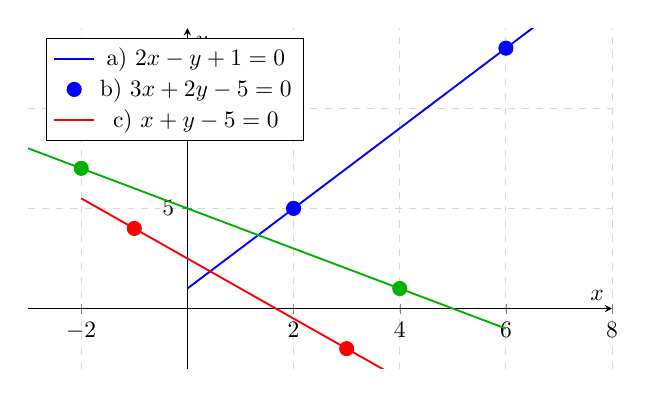
\begin{tikzpicture}[scale=0.85]
\begin{axis}[
    width=0.85\textwidth,
    height=0.55\textwidth,
    axis lines=middle,
    xlabel={$x$},
    ylabel={$y$},
    xmin=-3, xmax=8,
    ymin=-3, ymax=14,
    grid=major,
    grid style={dashed, gray!30},
    legend pos=north west,
]

% Inciso a)
\addplot[thick, color=blue, domain=0:7] {2*x + 1};
\addplot[only marks, mark=*, mark size=3pt, color=blue] coordinates {(2,5) (6,13)};
\addlegendentry{a) $2x - y + 1 = 0$}

% Inciso b)
\addplot[thick, color=red, domain=-2:4] {-1.5*x + 2.5};
\addplot[only marks, mark=*, mark size=3pt, color=red] coordinates {(-1,4) (3,-2)};
\addlegendentry{b) $3x + 2y - 5 = 0$}

% Inciso c)
\addplot[thick, color=green!70!black, domain=-3:6] {-x + 5};
\addplot[only marks, mark=*, mark size=3pt, color=green!70!black] coordinates {(4,1) (-2,7)};
\addlegendentry{c) $x + y - 5 = 0$}

\end{axis}
\end{tikzpicture}
\end{center}
\end{solucion}

% ============================================
% EJERCICIO 6: Rectas paralelas
% ============================================

\begin{ejercicio}[Rectas paralelas - Nivel INTERMEDIO]
Para cada recta dada, encuentra la ecuación de la recta paralela que pasa por el punto indicado:

\textbf{a)} Recta: $2x + 3y - 6 = 0$; Punto: $P(3, 4)$

\textbf{b)} Recta: $y = -4x + 7$; Punto: $Q(-1, 2)$

\textbf{c)} Recta: $x - 5y + 10 = 0$; Punto: $R(0, 0)$
\end{ejercicio}

\begin{solucion}
\textbf{Inciso a):}

\textbf{Paso 1:} Encontramos la pendiente de la recta dada:
\[
2x + 3y - 6 = 0 \quad \Rightarrow \quad 3y = -2x + 6 \quad \Rightarrow \quad y = -\frac{2}{3}x + 2
\]
Por lo tanto, $m_1 = -\frac{2}{3}$.

\textbf{Paso 2:} La recta paralela tiene la misma pendiente: $m_2 = -\frac{2}{3}$.

\textbf{Paso 3:} Forma punto-pendiente con $P(3, 4)$:
\begin{align*}
y - 4 &= -\frac{2}{3}(x - 3) \\
y - 4 &= -\frac{2}{3}x + 2 \\
y &= -\frac{2}{3}x + 6
\end{align*}

\textbf{Paso 4:} Forma general (multiplicamos por 3):
\[
3y = -2x + 18 \quad \Rightarrow \quad 2x + 3y - 18 = 0
\]

\textbf{Respuesta:} $\boxed{2x + 3y - 18 = 0}$ o $\boxed{y = -\frac{2}{3}x + 6}$

\textbf{Inciso b):}

\textbf{Paso 1:} La pendiente de la recta dada es $m_1 = -4$.

\textbf{Paso 2:} Recta paralela: $m_2 = -4$.

\textbf{Paso 3:} Con $Q(-1, 2)$:
\begin{align*}
y - 2 &= -4(x - (-1)) \\
y - 2 &= -4(x + 1) \\
y - 2 &= -4x - 4 \\
y &= -4x - 2
\end{align*}

\textbf{Respuesta:} $\boxed{y = -4x - 2}$ o $\boxed{4x + y + 2 = 0}$

\textbf{Inciso c):}

\textbf{Paso 1:} Pendiente de la recta dada:
\[
x - 5y + 10 = 0 \quad \Rightarrow \quad -5y = -x - 10 \quad \Rightarrow \quad y = \frac{1}{5}x + 2
\]
$m_1 = \frac{1}{5}$.

\textbf{Paso 2:} Recta paralela: $m_2 = \frac{1}{5}$.

\textbf{Paso 3:} Con $R(0, 0)$ (el origen):
\begin{align*}
y - 0 &= \frac{1}{5}(x - 0) \\
y &= \frac{1}{5}x
\end{align*}

\textbf{Paso 4:} Forma general (multiplicamos por 5):
\[
5y = x \quad \Rightarrow \quad x - 5y = 0
\]

\textbf{Respuesta:} $\boxed{x - 5y = 0}$ o $\boxed{y = \frac{1}{5}x}$
\end{solucion}

% ============================================
% EJERCICIO 7: Rectas perpendiculares
% ============================================

\begin{ejercicio}[Rectas perpendiculares - Nivel AVANZADO]
Para cada recta dada, encuentra la ecuación de la recta perpendicular que pasa por el punto indicado:

\textbf{a)} Recta: $3x - 4y + 12 = 0$; Punto: $P(6, 2)$

\textbf{b)} Recta: $y = 2x - 5$; Punto: $Q(4, 3)$

\textbf{c)} Recta: $x + 6y - 18 = 0$; Punto: $R(3, -1)$
\end{ejercicio}

\begin{solucion}
\textbf{Inciso a):}

\textbf{Paso 1:} Pendiente de la recta dada:
\[
3x - 4y + 12 = 0 \quad \Rightarrow \quad -4y = -3x - 12 \quad \Rightarrow \quad y = \frac{3}{4}x + 3
\]
$m_1 = \frac{3}{4}$.

\textbf{Paso 2:} Pendiente de la recta perpendicular:
\[
m_1 \cdot m_2 = -1 \quad \Rightarrow \quad \frac{3}{4} \cdot m_2 = -1 \quad \Rightarrow \quad m_2 = -\frac{4}{3}
\]

\textbf{Paso 3:} Con $P(6, 2)$:
\begin{align*}
y - 2 &= -\frac{4}{3}(x - 6) \\
y - 2 &= -\frac{4}{3}x + 8 \\
y &= -\frac{4}{3}x + 10
\end{align*}

\textbf{Paso 4:} Forma general (multiplicamos por 3):
\[
3y = -4x + 30 \quad \Rightarrow \quad 4x + 3y - 30 = 0
\]

\textbf{Respuesta:} $\boxed{4x + 3y - 30 = 0}$ o $\boxed{y = -\frac{4}{3}x + 10}$

\textbf{Inciso b):}

\textbf{Paso 1:} $m_1 = 2$.

\textbf{Paso 2:} Perpendicular:
\[
m_2 = -\frac{1}{2}
\]

\textbf{Paso 3:} Con $Q(4, 3)$:
\begin{align*}
y - 3 &= -\frac{1}{2}(x - 4) \\
y - 3 &= -\frac{1}{2}x + 2 \\
y &= -\frac{1}{2}x + 5
\end{align*}

\textbf{Respuesta:} $\boxed{y = -\frac{1}{2}x + 5}$ o $\boxed{x + 2y - 10 = 0}$

\textbf{Inciso c):}

\textbf{Paso 1:} Pendiente de la recta dada:
\[
x + 6y - 18 = 0 \quad \Rightarrow \quad 6y = -x + 18 \quad \Rightarrow \quad y = -\frac{1}{6}x + 3
\]
$m_1 = -\frac{1}{6}$.

\textbf{Paso 2:} Perpendicular:
\[
m_2 = -\frac{1}{m_1} = -\frac{1}{-\frac{1}{6}} = 6
\]

\textbf{Paso 3:} Con $R(3, -1)$:
\begin{align*}
y - (-1) &= 6(x - 3) \\
y + 1 &= 6x - 18 \\
y &= 6x - 19
\end{align*}

\textbf{Respuesta:} $\boxed{y = 6x - 19}$ o $\boxed{6x - y - 19 = 0}$

\begin{center}
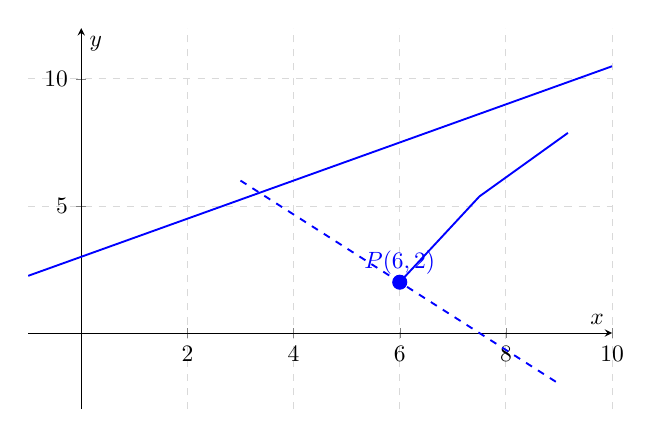
\begin{tikzpicture}[scale=0.85]
\begin{axis}[
    width=0.85\textwidth,
    height=0.6\textwidth,
    axis lines=middle,
    xlabel={$x$},
    ylabel={$y$},
    xmin=-1, xmax=10,
    ymin=-3, ymax=12,
    grid=major,
    grid style={dashed, gray!30},
]

% Inciso a)
\addplot[thick, color=blue, domain=-1:10] {0.75*x + 3};
\addplot[thick, color=blue, dashed, domain=3:9] {-4/3*x + 10};
\addplot[only marks, mark=*, mark size=3pt, color=blue] coordinates {(6,2)};
\node[above, blue] at (axis cs:6,2) {$P(6,2)$};

% Ángulo recto en P
\draw[thick, blue] (axis cs:6,2) -- ++(0.5,0.375) -- ++(0.667,-0.5);

\end{axis}
\end{tikzpicture}
\end{center}

\begin{nota}
Para verificar que dos rectas son perpendiculares, multiplica sus pendientes: el resultado debe ser $-1$.

Ejemplo inciso a): $m_1 \cdot m_2 = \frac{3}{4} \cdot \left(-\frac{4}{3}\right) = -\frac{12}{12} = -1$ ✓
\end{nota}
\end{solucion}

% ============================================
% EJERCICIO 8: Intersección de rectas
% ============================================

\begin{ejercicio}[Intersección de rectas - Nivel AVANZADO]
Encuentra el punto de intersección de los siguientes pares de rectas:

\textbf{a)} $L_1: 2x + y = 10$ y $L_2: x - y = 2$

\textbf{b)} $L_1: 3x - 2y = 6$ y $L_2: x + 4y = 14$

\textbf{c)} $L_1: y = 2x - 3$ y $L_2: y = -x + 6$
\end{ejercicio}

\begin{solucion}
\textbf{Inciso a):}

\textbf{Paso 1:} Tenemos el sistema:
\begin{align*}
2x + y &= 10 \quad \text{...(1)} \\
x - y &= 2 \quad \text{...(2)}
\end{align*}

\textbf{Paso 2:} Sumamos (1) + (2) para eliminar $y$:
\[
3x = 12 \quad \Rightarrow \quad x = 4
\]

\textbf{Paso 3:} Sustituimos en (2):
\[
4 - y = 2 \quad \Rightarrow \quad y = 2
\]

\textbf{Paso 4:} Verificamos en (1):
\[
2(4) + 2 = 8 + 2 = 10 \quad \checkmark
\]

\textbf{Respuesta:} $\boxed{(4, 2)}$

\textbf{Inciso b):}

\textbf{Paso 1:} Sistema:
\begin{align*}
3x - 2y &= 6 \quad \text{...(1)} \\
x + 4y &= 14 \quad \text{...(2)}
\end{align*}

\textbf{Paso 2:} De (2): $x = 14 - 4y$

\textbf{Paso 3:} Sustituimos en (1):
\begin{align*}
3(14 - 4y) - 2y &= 6 \\
42 - 12y - 2y &= 6 \\
-14y &= -36 \\
y &= \frac{36}{14} = \frac{18}{7}
\end{align*}

\textbf{Paso 4:} Sustituimos en $x = 14 - 4y$:
\[
x = 14 - 4 \cdot \frac{18}{7} = 14 - \frac{72}{7} = \frac{98 - 72}{7} = \frac{26}{7}
\]

\textbf{Respuesta:} $\boxed{\left(\frac{26}{7}, \frac{18}{7}\right) \approx (3.71, 2.57)}$

\textbf{Inciso c):}

\textbf{Paso 1:} Igualamos las dos ecuaciones:
\[
2x - 3 = -x + 6
\]

\textbf{Paso 2:} Resolvemos:
\begin{align*}
3x &= 9 \\
x &= 3
\end{align*}

\textbf{Paso 3:} Sustituimos en $y = 2x - 3$:
\[
y = 2(3) - 3 = 3
\]

\textbf{Paso 4:} Verificamos en $y = -x + 6$:
\[
y = -(3) + 6 = 3 \quad \checkmark
\]

\textbf{Respuesta:} $\boxed{(3, 3)}$

\begin{center}
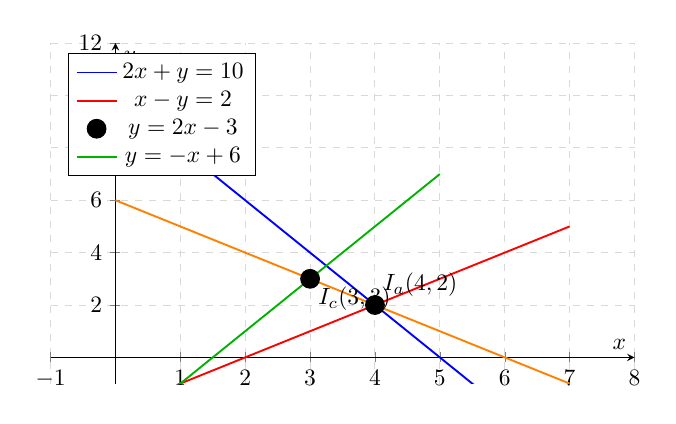
\begin{tikzpicture}[scale=0.85]
\begin{axis}[
    width=0.85\textwidth,
    height=0.55\textwidth,
    axis lines=middle,
    xlabel={$x$},
    ylabel={$y$},
    xmin=-1, xmax=8,
    ymin=-1, ymax=12,
    grid=major,
    grid style={dashed, gray!30},
    legend pos=north west,
]

% Inciso a)
\addplot[thick, color=blue, domain=0:6] {10 - 2*x};
\addplot[thick, color=red, domain=0:7] {x - 2};
\addplot[only marks, mark=*, mark size=4pt, color=black] coordinates {(4,2)};
\node[above right] at (axis cs:4,2) {$I_a(4,2)$};
\addlegendentry{$2x + y = 10$}
\addlegendentry{$x - y = 2$}

% Inciso c)
\addplot[thick, color=green!70!black, domain=0:5] {2*x - 3};
\addplot[thick, color=orange, domain=0:7] {-x + 6};
\addplot[only marks, mark=*, mark size=4pt, color=black] coordinates {(3,3)};
\node[below right] at (axis cs:3,3) {$I_c(3,3)$};
\addlegendentry{$y = 2x - 3$}
\addlegendentry{$y = -x + 6$}

\end{axis}
\end{tikzpicture}
\end{center}
\end{solucion}

% ============================================
% EJERCICIO 9: Aplicación en ingeniería civil
% ============================================

\begin{ejercicio}[Aplicación en ingeniería civil - Nivel AVANZADO]
Un ingeniero civil está diseñando el trazado de dos carreteras que se intersectan. La primera carretera sigue la ecuación $y = \frac{1}{2}x + 2$ y la segunda sigue $y = -\frac{2}{3}x + 10$ (coordenadas en kilómetros).

\textbf{a)} Encuentra el punto de intersección (donde se construirá una rotonda).

\textbf{b)} Calcula la distancia de la intersección al origen.

\textbf{c)} Una tercera carretera perpendicular a la primera debe pasar por la intersección. Encuentra su ecuación.

\textbf{d)} ¿En qué punto esta tercera carretera cruza el eje $x$?
\end{ejercicio}

\begin{solucion}
\textbf{Parte a):}

Igualamos las ecuaciones:
\begin{align*}
\frac{1}{2}x + 2 &= -\frac{2}{3}x + 10 \\
\frac{1}{2}x + \frac{2}{3}x &= 8
\end{align*}

MCM de 2 y 3 es 6:
\begin{align*}
\frac{3x + 4x}{6} &= 8 \\
7x &= 48 \\
x &= \frac{48}{7} \approx 6.86
\end{align*}

Sustituimos en $y = \frac{1}{2}x + 2$:
\[
y = \frac{1}{2} \cdot \frac{48}{7} + 2 = \frac{24}{7} + 2 = \frac{24 + 14}{7} = \frac{38}{7} \approx 5.43
\]

\textbf{Respuesta:} $\boxed{I\left(\frac{48}{7}, \frac{38}{7}\right) \approx (6.86, 5.43)}$

\textbf{Parte b):}

Distancia del origen $(0, 0)$ a $I$:
\[
d = \sqrt{\left(\frac{48}{7}\right)^2 + \left(\frac{38}{7}\right)^2} = \frac{1}{7}\sqrt{48^2 + 38^2} = \frac{1}{7}\sqrt{2304 + 1444} = \frac{\sqrt{3748}}{7}
\]

Simplificamos:
\[
\sqrt{3748} = \sqrt{4 \cdot 937} = 2\sqrt{937} \approx 61.21
\]

\[
d \approx \frac{61.21}{7} \approx 8.74 \text{ km}
\]

\textbf{Respuesta:} $\boxed{d \approx 8.74 \text{ km}}$

\textbf{Parte c):}

La primera carretera tiene $m_1 = \frac{1}{2}$.

La tercera carretera es perpendicular:
\[
m_3 = -\frac{1}{m_1} = -2
\]

Pasa por $I\left(\frac{48}{7}, \frac{38}{7}\right)$:
\begin{align*}
y - \frac{38}{7} &= -2\left(x - \frac{48}{7}\right) \\
y - \frac{38}{7} &= -2x + \frac{96}{7} \\
y &= -2x + \frac{96 + 38}{7} \\
y &= -2x + \frac{134}{7}
\end{align*}

\textbf{Respuesta:} $\boxed{y = -2x + \frac{134}{7}}$ o aproximadamente $\boxed{y = -2x + 19.14}$

\textbf{Parte d):}

Cuando $y = 0$:
\begin{align*}
0 &= -2x + \frac{134}{7} \\
2x &= \frac{134}{7} \\
x &= \frac{134}{14} = \frac{67}{7} \approx 9.57
\end{align*}

\textbf{Respuesta:} $\boxed{\left(\frac{67}{7}, 0\right) \approx (9.57, 0)}$

\begin{center}
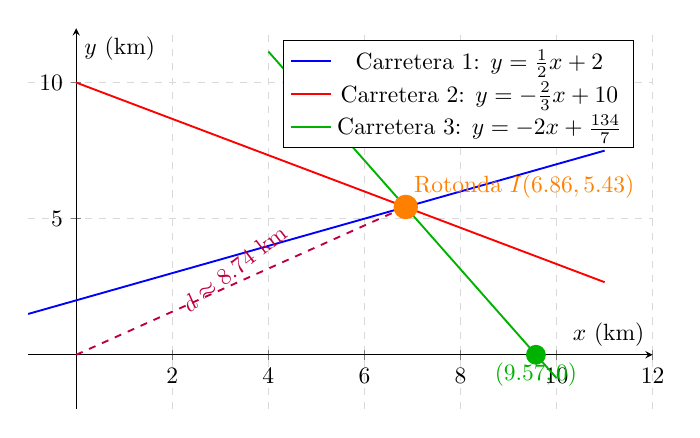
\begin{tikzpicture}[scale=0.85]
\begin{axis}[
    width=0.9\textwidth,
    height=0.6\textwidth,
    axis lines=middle,
    xlabel={$x$ (km)},
    ylabel={$y$ (km)},
    xmin=-1, xmax=12,
    ymin=-2, ymax=12,
    grid=major,
    grid style={dashed, gray!30},
    legend pos=north east,
]

% Primera carretera
\addplot[thick, color=blue, domain=-1:11] {0.5*x + 2};
\addlegendentry{Carretera 1: $y = \frac{1}{2}x + 2$}

% Segunda carretera
\addplot[thick, color=red, domain=0:11] {-2/3*x + 10};
\addlegendentry{Carretera 2: $y = -\frac{2}{3}x + 10$}

% Tercera carretera
\addplot[thick, color=green!70!black, domain=4:10] {-2*x + 134/7};
\addlegendentry{Carretera 3: $y = -2x + \frac{134}{7}$}

% Intersección
\addplot[only marks, mark=*, mark size=5pt, color=orange] coordinates {(6.86,5.43)};
\node[above right, orange] at (axis cs:6.86,5.43) {Rotonda $I(6.86, 5.43)$};

% Punto en eje x
\addplot[only marks, mark=*, mark size=4pt, color=green!70!black] coordinates {(9.57,0)};
\node[below, green!70!black] at (axis cs:9.57,0) {$(9.57, 0)$};

% Línea del origen a la intersección
\addplot[dashed, thick, color=purple] coordinates {(0,0) (6.86,5.43)};
\node[above, rotate=38, purple] at (axis cs:3.5,2.7) {$d \approx 8.74$ km};

\end{axis}
\end{tikzpicture}
\end{center}
\end{solucion}

% ============================================
% EJERCICIO 10: Problema integral
% ============================================

\begin{ejercicio}[Problema integral de geometría analítica - Nivel AVANZADO]
Tres vértices de un paralelogramo son $A(1, 2)$, $B(5, 4)$, y $C(7, 8)$.

\textbf{a)} Encuentra las coordenadas del cuarto vértice $D$.

\textbf{b)} Calcula el perímetro del paralelogramo.

\textbf{c)} Encuentra las ecuaciones de las dos diagonales.

\textbf{d)} Determina el punto de intersección de las diagonales y verifica que es el punto medio de ambas.
\end{ejercicio}

\begin{solucion}
\textbf{Parte a):}

En un paralelogramo, las diagonales se bisectan mutuamente (se cortan en su punto medio).

Las dos diagonales son $AC$ y $BD$.

Punto medio de $AC$:
\[
M_{AC} = \left(\frac{1+7}{2}, \frac{2+8}{2}\right) = (4, 5)
\]

Este también debe ser el punto medio de $BD$. Sea $D(x, y)$:
\[
\left(\frac{5+x}{2}, \frac{4+y}{2}\right) = (4, 5)
\]

Por lo tanto:
\begin{align*}
\frac{5+x}{2} &= 4 \quad \Rightarrow \quad 5+x = 8 \quad \Rightarrow \quad x = 3 \\
\frac{4+y}{2} &= 5 \quad \Rightarrow \quad 4+y = 10 \quad \Rightarrow \quad y = 6
\end{align*}

\textbf{Respuesta:} $\boxed{D(3, 6)}$

\textbf{Parte b):}

Calculamos las longitudes de los lados:

Lado $AB$:
\[
|AB| = \sqrt{(5-1)^2 + (4-2)^2} = \sqrt{16 + 4} = \sqrt{20} = 2\sqrt{5}
\]

Lado $BC$:
\[
|BC| = \sqrt{(7-5)^2 + (8-4)^2} = \sqrt{4 + 16} = \sqrt{20} = 2\sqrt{5}
\]

Lado $CD$ (debe ser igual a $AB$):
\[
|CD| = \sqrt{(3-7)^2 + (6-8)^2} = \sqrt{16 + 4} = \sqrt{20} = 2\sqrt{5}
\]

Lado $DA$ (debe ser igual a $BC$):
\[
|DA| = \sqrt{(1-3)^2 + (2-6)^2} = \sqrt{4 + 16} = \sqrt{20} = 2\sqrt{5}
\]

Perímetro:
\[
P = 4 \times 2\sqrt{5} = 8\sqrt{5} \approx 17.89 \text{ unidades}
\]

\textbf{Respuesta:} $\boxed{P = 8\sqrt{5} \approx 17.89 \text{ unidades}}$

\textbf{Observación:} En este caso particular, ¡todos los lados son iguales! Esto significa que el paralelogramo es en realidad un \textbf{rombo}.

\textbf{Parte c):}

\textbf{Diagonal AC:}

Pendiente:
\[
m_{AC} = \frac{8-2}{7-1} = \frac{6}{6} = 1
\]

Ecuación con $A(1, 2)$:
\[
y - 2 = 1(x - 1) \quad \Rightarrow \quad y = x + 1
\]

\textbf{Diagonal BD:}

Pendiente:
\[
m_{BD} = \frac{6-4}{3-5} = \frac{2}{-2} = -1
\]

Ecuación con $B(5, 4)$:
\[
y - 4 = -1(x - 5) \quad \Rightarrow \quad y = -x + 9
\]

\textbf{Respuesta:}
\begin{itemize}
    \item Diagonal $AC$: $\boxed{y = x + 1}$
    \item Diagonal $BD$: $\boxed{y = -x + 9}$
\end{itemize}

\textbf{Parte d):}

Intersección (igualamos):
\begin{align*}
x + 1 &= -x + 9 \\
2x &= 8 \\
x &= 4
\end{align*}

Sustituimos:
\[
y = 4 + 1 = 5
\]

Punto de intersección: $I(4, 5)$

\textbf{Verificación:}

Punto medio de $AC$:
\[
M_{AC} = \left(\frac{1+7}{2}, \frac{2+8}{2}\right) = (4, 5) \quad \checkmark
\]

Punto medio de $BD$:
\[
M_{BD} = \left(\frac{5+3}{2}, \frac{4+6}{2}\right) = (4, 5) \quad \checkmark
\]

¡Ambos coinciden con el punto de intersección!

\textbf{Respuesta:} $\boxed{I(4, 5)}$ es el punto de intersección y es el punto medio de ambas diagonales. ✓

\begin{center}
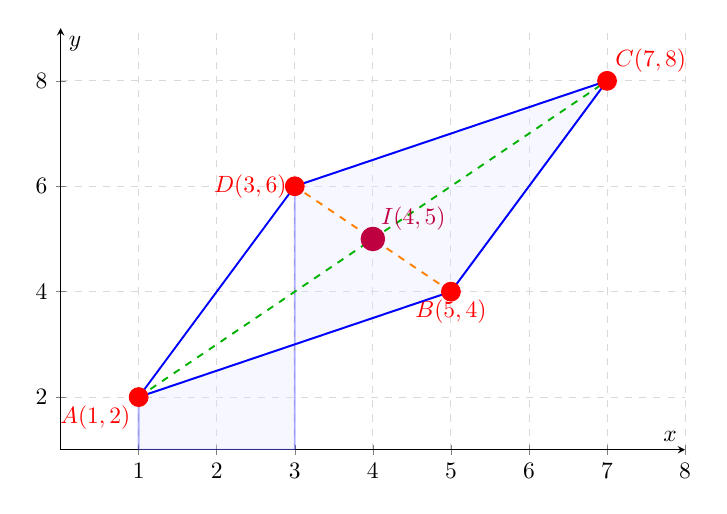
\begin{tikzpicture}[scale=0.85]
\begin{axis}[
    width=0.9\textwidth,
    height=0.65\textwidth,
    axis lines=middle,
    xlabel={$x$},
    ylabel={$y$},
    xmin=0, xmax=8,
    ymin=1, ymax=9,
    grid=major,
    grid style={dashed, gray!30},
]

% Paralelogramo ABCD
\addplot[thick, color=blue, fill=blue!10, opacity=0.3] coordinates {(1,2) (5,4) (7,8) (3,6)} \closedcycle;

% Vértices
\addplot[only marks, mark=*, mark size=4pt, color=red] coordinates {(1,2) (5,4) (7,8) (3,6)};
\node[below left, red] at (axis cs:1,2) {$A(1,2)$};
\node[below, red] at (axis cs:5,4) {$B(5,4)$};
\node[above right, red] at (axis cs:7,8) {$C(7,8)$};
\node[left, red] at (axis cs:3,6) {$D(3,6)$};

% Diagonales
\addplot[thick, color=green!70!black, dashed] coordinates {(1,2) (7,8)};
\addplot[thick, color=orange, dashed] coordinates {(5,4) (3,6)};

% Punto de intersección
\addplot[only marks, mark=*, mark size=5pt, color=purple] coordinates {(4,5)};
\node[above right, purple] at (axis cs:4,5) {$I(4,5)$};

% Lados del paralelogramo
\addplot[thick, color=blue] coordinates {(1,2) (5,4)};
\addplot[thick, color=blue] coordinates {(5,4) (7,8)};
\addplot[thick, color=blue] coordinates {(7,8) (3,6)};
\addplot[thick, color=blue] coordinates {(3,6) (1,2)};

\end{axis}
\end{tikzpicture}
\end{center}

\begin{nota}
Este paralelogramo es en realidad un \textbf{rombo} porque todos sus lados tienen la misma longitud ($2\sqrt{5}$). Además, las diagonales son perpendiculares ($m_1 \cdot m_2 = 1 \cdot (-1) = -1$), lo cual es otra propiedad característica de los rombos.
\end{nota}
\end{solucion}
